% LaTeX Language and campus name and format package
\documentclass[es,gi]{ifirak}
% ERABILIKO DIREN PAKETEAK %

% listings pakage is for code formating
\usepackage{listings}
% Paquete for acents and other special characters
% It is not necesary to use all this packages add or remove those you are interested on
\usepackage[utf8]{inputenc}
\usepackage{colortbl}
\usepackage[table]{xcolor}
\usepackage{graphicx}
\usepackage{wrapfig}
\usepackage{amsfonts}
\usepackage{makeidx}
\usepackage{multicol}
% Definition of colors
\definecolor{darkgreen}{rgb}{0,0.5,0}
\definecolor{lightgray}{rgb}{0.95,0.95,0.95}
\definecolor{gray}{rgb}{0.85,0.85,0.85}
\definecolor{white}{rgb}{1,1,1}
\definecolor{purple}{rgb}{0.51,0,0.25}
\definecolor{orange}{rgb}{0.255,0.178,0.102}
%Definition of style for code
\lstdefinestyle{customc}{
	belowcaptionskip=1\baselineskip,
	breaklines=true,
	tabsize=4,
	language=C,
	showstringspaces=false,
	basicstyle=\footnotesize\ttfamily,
	keywordstyle=\bfseries\color{darkgreen},
	commentstyle=\itshape\color{purple},
	identifierstyle=\color{blue},
	stringstyle=\color{orange},
	backgroundcolor=\color{lightgray},
}
\lstset{language=C,escapechar=@,style=customc}
\DeclareMathSizes{10}{10}{10}{10}
\newenvironment{Figure}
  {\par\medskip\noindent\minipage{\columnwidth}}
  {\endminipage\par\medskip}
\IfFileExists{upquote.sty}{\usepackage{upquote}}{}
\begin{document}

% Course year
\ikasturtea{2015 - 2016}
% Subject or course name
\irakasgaia{Sistemas de Cómputo Paralelo}
% Title
\title{Puzle, Parte 1}
% Name of Author
\author{Mikel Dalmau}

\maketitle

\setlength{\columnsep}{1cm}
%\section{Código}
\begin{multicols}{2}
\section{Comunicaciones colectivas}
\paragraph{}	
En la comunicación entre un grupo de individuos, existen mecanismos que permiten una comunicación más eficiente. En este trabajo en el apartado 1.1 \textit{Comunicación en forma de árbol} se muestran varios modelos de comunicación compuestos por árboles.\\

En MPI, la comunicación colectiva consiste en una serie de funciones que sirven para que un grupo de procesos se comuniquen entre ellos. En el apartado 1.2 \textit{Comunicaciones colectivas frente a comunicaciones Punto a Punto} se muestran las diferencias principales entre las funciones de comunicación colectiva y las de punto a punto. En el apartado 1.3 \emph{Funciones de Comunicación Colectiva en MPI} se describen las funciones más utilizadas y sus parámetros.\\
\subsection{Comunicación en forma de árbol}
\paragraph{}
En \cite{key-1} se describe esta forma de comunicación, mostrando como ejemplo un problema de suma \textit{one-to-all}. Aunque inicialmente pueda parecer que no mejora demasiado, ya que la mitad de los nodos realizan las mismas comunicaciones que realizarían punto a punto(esto es, cuando todos los nodos envían su valor a un único nodo), mejora considerablemente reduciendo la cantidad de recepciones y sumas que tiene que realizar el nodo líder. 
\paragraph{}
En el ejemplo de la imagen, el nodo 0 pasa de realizar \textit{n-1} recepciones y sumas a realizar 3 recepciones y sumas, esto es, la altura del árbol $log_2\;n$($log_d\;n$ en el caso general, siendo \textit{d} el grado de árbol). De esta forma la carga de trabajo de los nodos crece logarítmica-mente con el número de procesadores, la mejora es notable frente al crecimiento lineal de la comunicación centralizada.

\begin{Figure}
	\centering
	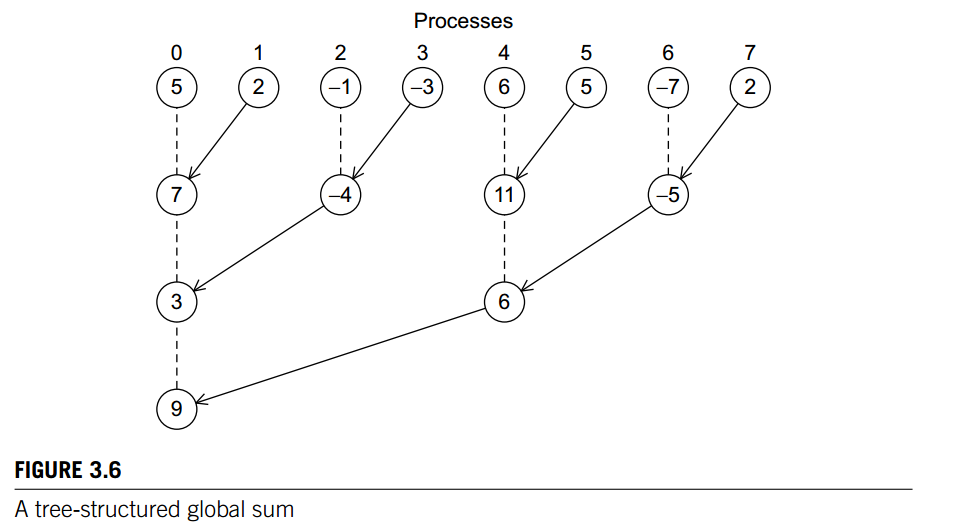
\includegraphics[width=1\columnwidth]{TreeSum.png}
	%\caption{Imágen extraída de \cite{key-1} , Apartado 3.4.1 .}  	    
	\label{figure}
\end{Figure}

El mismo modelo invertido se puede utilizar para comunicación \textit{one-to-all}.
\begin{Figure}
	\centering
		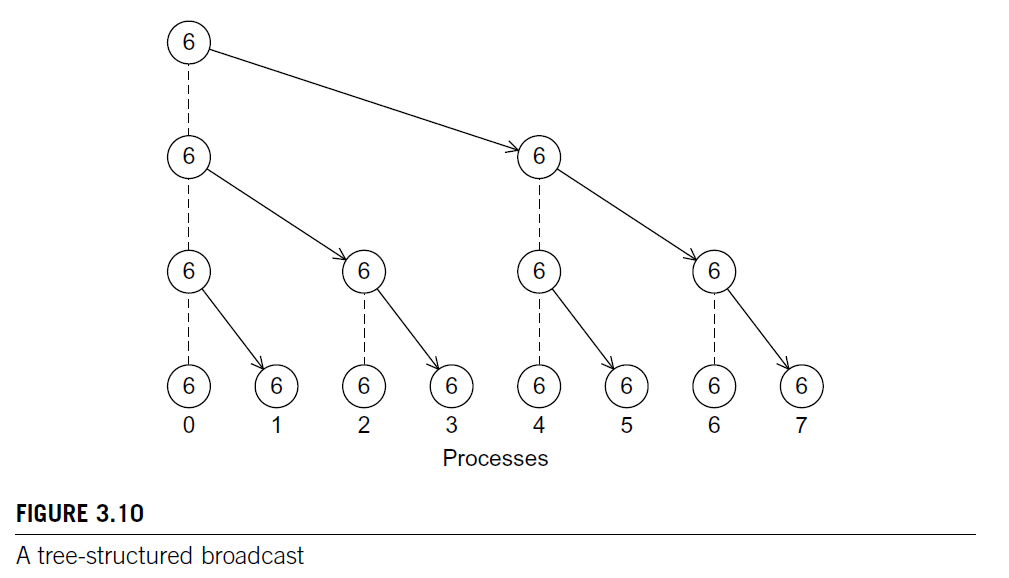
\includegraphics[width=1\columnwidth]{TreeBroadcast.png}
		%\caption{Imágen extraída de \cite{key-1} , Apartado 3.4.5 .}						\label{figure}
\end{Figure}

Este último ejemplo muestra un modelo de comunicación all-to-all en el que se construyen n árboles siendo cada nodo raíz de uno de ellos. 
\begin{Figure}
	\centering
		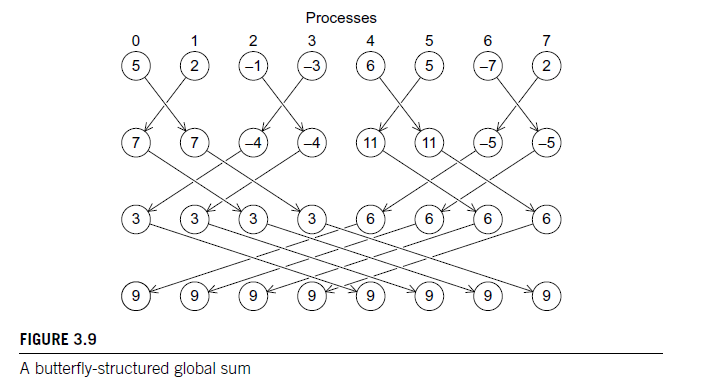
\includegraphics[width=1\columnwidth]{Butterfly.png}
		%\caption{Imágen extraída de \cite{key-1} , Apartado 3.4.5 .}						\label{figure}
\end{Figure}

\paragraph{}
El problema de este modelo de comunicación es la dificultad de programarlo, existen incontables maneras distintas de hacerlo pero no sabríamos cual es la mejor, para que tipos y tamaños de problemas cual es la óptima. En \cite{key-2} se sugiere también el uso de árboles de profundidad logarítmica para la comunicación, pero tampoco indican o desconocen si las funciones MPI hacen uso de ellos.
\subsection{Comunicaciones colectivas frente a comunicaciones Punto a Punto}

\begin{itemize}
\item[1.] Todos los procesos en el comunicador deben llamar a la misma función colectiva independientemente del tipo de comunicación que se realice. Mientras en la comunicación punto a punto queda definido por la llamada quien es emisor y quien es receptor, MPI\_Recv y MPI\_Send.
\item[2.] Todos los procesos en el comunicador tienen que tener los parámetros compatibles, esto es, si en una llamada MPI\_Reduce dos procesos tiene \textit{root} distinto el programa va a fallar.
\item[3.] Las funciones de comunicación punto a punto se conectan mediante etiquetas (\textit{tags}) y comunicadores, en las colectivas solamente mediante comunicadores y el orden en el que son llamadas.
\item[4.] Otra restricción que las funciones de comunicación punto a punto no tienen es que la cantidad de datos enviados en el bufer tiene que coincidir exactamente con la esperada en el destino.
\item[5.] No exiten funciones de comunicación colectivas que no sean bloqueante, todas utilizan la función Barrier para asegurar las sincronización de los datos.

\end{itemize} 
\subsection{Funciones de Comunicación Colectiva en MPI}
\paragraph{}
Podemos dividir las funciones de comunicación colectiva en función del tipo de comunicación que realizan y también en función del tipo de dato que manejan ya que así las distingue MPI.

\begin{itemize}
\item[-] \textit{all-to-one}:
	\begin{itemize}
		\item[•] MPI\_REDUCE
		\item[•] MPI\_GATHER
	\end{itemize}
\item[-] \textit{one-to-all}
    \begin{itemize}
		\item[•] MPI\_BCAST
		\item[•] MPI\_SCATTER
	\end{itemize}
\item[-] \textit{all-to-all}
	 \begin{itemize}
	    \item[•] MPI\_ALLREDUCE
		\item[•] MPI\_ALLGATHER
		\item[•] MPI\_ALLTOALL
		\item[•] MPI\_REDUCE\_SCATTER
	\end{itemize}
\item[-] \textit{\textit{all-to-some}}
	\begin{itemize}
		\item[•] MPI\_SCAN
	\end{itemize}
\end{itemize}

Respecto al tipo de dato que manejan, MPI dispone de las \textit{vector variant} de las funciones vistas; MPI\_GATHERV, MPI\_SCATTERV, MPI\_ALLGATHERV, MPI\_ALLTOALLV.\\

Estas funciones se diferencian por...\\

Respecto a las funciones ALL, en estas los parámetros son idénticos que los de sus semejantes con la excepción de que sobra el parámetro \textit{root} ya que todos recibirán el mensaje.

\subsubsection{MPI\_Bcast}
\paragraph{}


\begin{verbatim}
NAME
     MPI_Bcast -  Broadcasts a message from the 
     process with rank "root" to all other processes
     of the communicator

SYNOPSIS
     int MPI_Bcast( void *buffer, int count, 
     MPI_Datatype datatype, int root,
           				MPI_Comm comm )
       
\end{verbatim}

\subsubsection{MPI\_Reduce}
\paragraph{}

\begin{verbatim}
NAME
     MPI_Reduce -  Reduces values on all
            processes to a single value

SYNOPSIS
     int MPI_Reduce(MPICH2_CONST void *sendbuf, 
     void *recvbuf, int count, MPI_Datatype 
     datatype, MPI_Op op, int root, MPI_Comm comm)
     
\end{verbatim}

Es de especial interés el parámetro \textit{op} que define el tipo de operación a realizar. Existen los siguientes tipos de operaciones:

\begin{center}
	\begin{tabular}{|l|l|}
		\hline
		\cellcolor{gray}Operation Value & \cellcolor{gray}Meaning \\
		\hline
		MPI\_MAX & Máximo\\
		MPI\_MIN & Mínimo\\
		MPI\_SUM & Suma\\
		MPI\_PROD & Producto\\
		MPI\_LAND & And lógico	\\
		MPI\_BAND & And binario	\\
		MPI\_LOR & Or lógico\\
		MPI\_BOR & Or binario	\\
		MPI\_LXOR & Or exclusivo lógico	\\
		MPI\_BXOR & Or exclusivo binario	\\
		MPI\_MAXLOC & Máximo y su dirección	\\
		MPI\_MINLOC & Mínimo y su dirección	\\
		\hline
	\end{tabular}
\end{center}

\subsubsection{MPI\_Scatter}


\subsubsection{MPI\_Gather}



\pagebreak
\section{Ejercicios}

\subsection{P1.1}
\paragraph{}
Hay que repartir un vector de N elementos entre npr procesos. Completa el programa serie \textit{P11-distribute0.c}, para que genere el tamaño de cada trozo del vector y el desplazamiento desde el origen del vector al comienzo de cada trozo, en estos dos casos: 

\begin{itemize}
\item[\textbf{a.}] los posibles restos se añaden al último trozo
\item[\textbf{b.}] los posibles restos se añaden uno a uno a diferentes trozos
\end{itemize}

\hline

\paragraph{a.}
Inicialmente calculo Nloc y remainder.
\begin{lstlisting}
//Compute Nloc and remainder
Nloc = floor((double)N/(double)npr);
remainder = N - Nloc*npr;
\end{lstlisting}
\paragraph{}
Este caso es sencillo y se resuelve con el siguiente bucle y las asignaciones finales.
\begin{lstlisting}
//We distribute the work among the procesesses
for(i=0; i<npr-1; i++){
	size[i] = Nloc;
	shift[i] = i*Nloc;
}
//Finally we charge the last process with the remainder
size[npr-1] = Nloc + remainder;
shift[npr-1] = (npr-1)*Nloc;
\end{lstlisting}

\paragraph{b.}
En este segundo caso he comenzado distribuyendo la carga del resto entre los primeros procesadores, luego,
las cargas distintas entre procesos no permiten el cálculo de shift usado anteriormente, por lo que tomo las referencias de tamaño y shift calculadas en la anterior iteración para calcular el shift, sabemos donde empezamos porque sabemos dónde termina el anterior.

\begin{lstlisting}
//Value asignment to first process  
size2[0] = Nloc;
shift2[0] = 0; 

//Distribution of the remainder among the first processes 
i = 0;
while(remainder){
	size2[i] += 1;
	remainder -= 1;
	i++;
}
	
//Distribute the rest of the vector among the processes
for(i=1; i<npr; i++){
	size2[i] += Nloc;
	shift2[i] = shift2[(i-1)] + size2[(i-1)];
}
\end{lstlisting}

\subsection{P1.2}

El programa \textit{P12-inteser.c} calcula el valor de una integral mediante el conocido método de sumar las áreas de n trapecios bajo la curva que representa una función. A mayor valor de n, más preciso el resultado.\\

Completa el programa MPI \textit{P12-inteser.c} para realizar esa misma función entre P procesos, utilizando funciones de comunicación colectiva. Compara el resultado con el de la versión serie.\\

\hline

\paragraph{}
Para resolver el problema es necesario modificar la función Read\_data, encargada de leer por pantalla los límites superior, inferior y número de evaluaciones de la función. Dado que todos los nodos no pueden utilizar la entrada estándar al mismo tiempo, limito la lectura a un único nodo y luego distribuyo los datos leídos entre el resto de procesos utilizando la función \textbf{MPI\_Bcast}.
\begin{lstlisting}
void Read_data(double* a_ptr, double* b_ptr, int* n_ptr, int pid){

  float a, b;
  float buf[3];
  
  if (pid == 0){
	printf("\n  Introduce a, b (limits) and n (num. of trap.)  \n");
	scanf("%f %f %d", &a, &b, n_ptr);
	buf[0] = a; 	
	buf[1] = b;
	buf[2] = (float)*n_ptr;
  }
  //Distribute read values
  MPI_Bcast(&buf,3,MPI_INT,0,MPI_COMM_WORLD);

  (*a_ptr)= (double)(buf[0]);
  (*b_ptr)= (double)(buf[1]);
  (*n_ptr)= (double)(buf[2]);
\end{lstlisting}

Tras realizar el cálculo del área correspondiente en cada proceso, es necesario sumarlas todas para obtener la integral en todo el intervalo. Esto puede realizarse en una única línea llamando a la función \textbf{MPI\_Reduce} con los siguientes parámetros.

\begin{lstlisting}
/* 
Adding the partial results,

  Description of parameters:
  sendbuf  - local result of integral
  recvbuf  - total result of integral
  count    - 1 element in send buffer per porcess
  datatype - We are using double precission
  op       - We will compute a sume
  root     - the process 0
  comm     - All the processes active 
*/
 MPI_Reduce(&resul_loc, &resul, 1, MPI_DOUBLE	, MPI_SUM, 0, MPI_COMM_WORLD);
\end{lstlisting}


\begin{thebibliography}{rules}
\bibitem{key-1} Pacheco P.:\textit{An Introduction to Parallel Programming}. Morgan Kaufmann,2011. Capítulo 3, apartado 4. 

\bibitem{key-2} Snir M., Otto S., Huss-Lederman S., Walker D., Dongarra J. \textit{MPI: The Complete Reference, Volume 1, The MPI Core.} The MIT PRess,1999. Capítulo 4.

\end{thebibliography}

\end{multicols}

\end{document}
